\documentclass[12pt, orivec]{article}
\usepackage{amsmath}
\usepackage{amssymb}     % for \rightsquigarrow
\usepackage{wasysym}
\usepackage[breakable]{tcolorbox}
\usepackage{ulem}
\usepackage{tikz-cd}		% commutative diagrams
\usepackage{tikz}
\usepackage{amsthm}
\usepackage[backend=biber,bibstyle=authoryear,citestyle=authoryear]{biblatex}
\bibliography{../AGI-book}

\newtheorem{theorem}{Theorem}

\ifdefined\chinchin
\usepackage[CJKspace]{xeCJK}
\setCJKmainfont[BoldFont=SimHei,ItalicFont=AR PL KaitiM GB]{SimSun}
\newcommand{\cc}[2]{#1}
\else
\newcommand{\cc}[2]{#2}
\fi

\newcommand{\code}   [1]{{\footnotesize{\ttfamily #1}}}
\newcommand{\tab}{\hspace*{2cm}}

\title{\cc{《计算范畴论》导读}{Computational category theory -- a tutorial}}
\author{甄景贤 {\footnotesize \ttfamily generic.intelligence@gmail.com}}

\begin{document}
\setlength{\parindent}{0pt}
\setlength{\parskip}{2.8ex plus0.8ex minus0.8ex}

\maketitle

\cc{恶补数学好几年之后,最近看懂了很多书。 《Computational category theory》 
}{
After a few years of bad mathematics, I have read a lot of books recently. Computational category theory
}
\cc{是 Rydeheard \& Burstall 1988 年的书,但至今还没有类似的课本。  
}{
is Rydeheard \& Burstall's 1988 book, but there are no newer textbooks on this topic.
}

\cc{我觉得这本书非常重要,因为它涉及到 \textbf{unification algorithm}。  现时人工智能中最关键的问题似乎是如何从 propositional logic(命题逻辑)过渡到 relational 或 first-order logic(一阶谓词逻辑),特别是如何找到高效率的学习算法。  关於 logic-based AI 的基础可以看看《AI --- a modern approach》 这本书。  
}{
I think this book is very important because it involves \textbf{unification algorithm}. The most critical issue in artificial intelligence seems to be how to transition from propositional logic to relational or first-order logic, especially how to find efficient learning algorithms. The basics of logic-based AI can be found in the book "AI --- a modern approach".
}

\cc{Unification algorithm(同一化算法)是 谓词逻辑 推导的核心算法。  将这个算法加进 命题逻辑 的推导算法(它叫消解法,resolution),就可以得到 谓词逻辑 的推导算法。  换句话说: unification + resolution = first-order deduction.
}{
The Unification algorithm is the core algorithm for predicate logic derivation. By adding this algorithm to the derivation algorithm of the propositional logic (which is called resolution), the derivation algorithm of the predicate logic can be obtained. In other words: unification + resolution = first-order deduction.
}

\cc{Unify 的意思是: 将两个 \textbf{逻辑项},透过 \textbf{variable substitution} 变成「一样」。  Variable substitution 是 谓词逻辑 的本质,\textbf{量词} $\forall$ 和 $\exists$ 就是作用在这些变量上。  所有初中生都懂得如何做「变量代入」,但它其实是一个很麻烦的动作,没有了它,谓词逻辑 就变成 命题逻辑。  虽然所有数学家都知道什么是 variable substitution,但它的精确描述,到了 1920-30 年代才开始出现。 例如 Sch\"{o}nfinkel 和 Curry 创造了 combinatory logic,Church 创造了 $\lambda$-calculus),他们的目的之一就是揭示「代入」的机制。 
}{
Unify means: Turn two \textbf{logical items} into "same" through \textbf{variable substitution}. Variable substitution is the essence of predicate logic, and \textbf{ quantifiers} $\forall$ and $\exists$ are applied to these variables. All junior high school students know how to do "variable substitution", but it is actually a very troublesome action. Without it, the predicate logic becomes propositional logic. Although all mathematicians know what variable substitution is, its precise description did not begin until the 1920s and 30s. For example, Sch\"{o}nfinkel and Curry created combinatory logic, and Church created $\lambda$-calculus. One of their purposes is to reveal the mechanism of "substitution".
}

\cc{Unification 的例子:
}{
Example of Unification:
}
\begin{equation}
\mbox{loves}(X,Y) = \mbox{loves}(\mbox{john}, \mbox{mary}) \quad \mbox{ with } \{ X/\mbox{john}, Y/\mbox{mary} \}
\end{equation}
\cc{(如果逻辑里面有 function symbols 可以更复杂)
}{
(If the function symbols in the logic can be more complicated)
}

\cc{Unifcation 算法最初由 Jacques Herbrand (1930) 提出,后经 J A Robinson (1965) 发明 resolution 算法,再将它们结合,应用到自动推理。 
}{
The Unifcation algorithm was originally proposed by Jacques Herbrand (1930), and the resolution algorithm was invented by J A Robinson (1965), which was then combined and applied to automatic reasoning.
}
\begin{equation}
\vcenter{\hbox{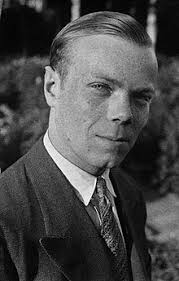
\includegraphics[scale=0.6]{Jacques-Herbrand.jpg}}} \quad
\vcenter{\hbox{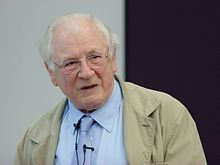
\includegraphics[scale=1.0]{John_Alan_Robinson.jpg}}} \nonumber
\end{equation}

\cc{在经典逻辑 AI 中,unification 是核心算法之一,但它的时间复习性并不是瓶颈。  笔者曾经研发过 higher-order unification,有开源代码在 GitHub.
}{
In classic logic AI, unification is one of the core algorithms, but its time review is not a bottleneck. I have developed higher-order unification and have open source code on GitHub.
}

\cc{以下是一个简单的 unification algorithm in Lisp,作者是 Peter Norvig: 
}{
The following is a simple unification algorithm in Lisp by Peter Norvig:
}
\begin{tcolorbox}[breakable]
\footnotesize
\ttfamily
\begin{verbatim}
;;; -*- Mode: Lisp; Syntax: Common-Lisp; -*-
;;; Code from Paradigms of Artificial Intelligence Programming
;;; Copyright (c) 1991 Peter Norvig

;;;; File unify.lisp: Unification functions

(requires "patmatch")

(defparameter *occurs-check* t "Should we do the occurs check?")

(defun unify (x y &optional (bindings no-bindings))
  "See if x and y match with given bindings."
  (cond ((eq bindings fail) fail)
        ((eql x y) bindings)
        ((variable-p x) (unify-variable x y bindings))
        ((variable-p y) (unify-variable y x bindings))
        ((and (consp x) (consp y))
         (unify (rest x) (rest y) 
                (unify (first x) (first y) bindings)))
        (t fail)))

(defun unify-variable (var x bindings)
  "Unify var with x, using (and maybe extending) bindings."
  (cond ((get-binding var bindings)
         (unify (lookup var bindings) x bindings))
        ((and (variable-p x) (get-binding x bindings))
         (unify var (lookup x bindings) bindings))
        ((and *occurs-check* (occurs-check var x bindings))
         fail)
        (t (extend-bindings var x bindings))))

(defun occurs-check (var x bindings)
  "Does var occur anywhere inside x?"
  (cond ((eq var x) t)
        ((and (variable-p x) (get-binding x bindings))
         (occurs-check var (lookup x bindings) bindings))
        ((consp x) (or (occurs-check var (first x) bindings)
                       (occurs-check var (rest x) bindings)))
        (t nil)))

(defun subst-bindings (bindings x)
  "Substitute the value of variables in bindings into x,
  taking recursively bound variables into account."
  (cond ((eq bindings fail) fail)
        ((eq bindings no-bindings) x)
        ((and (variable-p x) (get-binding x bindings))
         (subst-bindings bindings (lookup x bindings)))
        ((atom x) x)
        (t (reuse-cons (subst-bindings bindings (car x))
                       (subst-bindings bindings (cdr x))
                       x))))

(defun unifier (x y)
 "Return something that unifies with both x and y (or fail)."
 (subst-bindings (unify x y) x))
\end{verbatim}
\normalsize
\rmfamily
\end{tcolorbox}

\cc{从深度学习的角度考虑,问题是如何将 神经网络 算法 融合到 逻辑算法?  \uline{表面上看,这是两件截然不同的东西}。 笔者思考这个问题很多年,也提出过一些方案,但并不特别成功。 为了更明白 unification 的机制,我看了一些从范畴论角度处理 unification 的理论。
}{
From the perspective of deep learning, the question is how to integrate neural network algorithms into logic algorithms? \uline{On the surface, this is two very different things}. The author has been thinking about this issue for many years and has proposed some programs, but it is not particularly successful. In order to better understand the mechanism of unification, I have seen some theories dealing with unification from the perspective of category theory.
}

\cc{最早用范畴论角度研究 unification 的人是 Joseph Goguen (1941-2006),他发现了 unification 对应於范畴论中的 \textbf{co-equalizer} 概念:
}{
The first person to study unification from the perspective of category theory was Joseph Goguen (1941-2006), who discovered that unification corresponds to the concept of \textbf{co-equalizer} in category theory:
}
\begin{equation}
\vcenter{\hbox{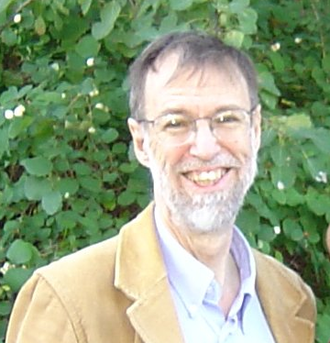
\includegraphics[scale=0.5]{Joseph-Goguen.png}}} \nonumber
\end{equation}
\cc{他写了一篇很详细的论文《What is unification? --- a categorical view of substitution, equation and solution》 (1989).
}{
He wrote a very detailed paper "What is unification? --- a categorical view of substitution, equation and solution" (1989).
}

\cc{首先介绍一下什么是 \textbf{计算} 范畴论。  范畴论很抽象(它关注在集合之间的\textbf{映射},而不是集合里面的\textbf{元素}),但计算是具体的。  关键是: 用 \textbf{types} 代表 范畴论里的 objects,\textbf{functions} 代表范畴论里的 morphisms。  换句话说,用 \textbf{函数式编程} 模拟范畴论,计算返回的结果是一些 functions。
}{
First introduce what is the \textbf{calculation} category theory. The category theory is abstract (it focuses on the \textbf{map} between collections, not the \textbf{element} in the collection), but the calculation is concrete. The key is: Use \textbf{types} to represent objects in category theory, and \textbf{functions} to represent morphisms in category theory. In other words, using \textbf{functional programming} to simulate category theory, the result of the calculation is some functions.
}

\begin{tcolorbox}
\cc{众所周知,Haskell 的前身是 ML,ML = Lisp + type system.  ML 也衍生了 OCaml = Objective Caml,而 Caml 的 CAM = categorical abstract machine.  CAM 是 Cartesian-closed category 和 combinatory logic 的结合。 (我暂时还不大清楚 CAM 的理论)
}{
As we all know, Haskell's predecessor is ML, ML = Lisp + type system. ML also derives OCaml = Objective Caml, and Caml's CAM = categorical abstract machine. CAM is a combination of Cartesian-closed category and combinatory logic. (I don't know the theory of CAM for the time being)
}
\end{tcolorbox}

\cc{在 Rydeheard \& Burstall 这本书里,用的语言是 ML。 例如: \\
}{
In the book Rydeheard \& Burstall, the language used is ML. E.g: \\
}
\tab 用 type \code{`o} 表示 objects,\\
\tab 用 type \code{`a} 表示 arrows,\\
\cc{那么 source 和 target 函数的类型就是 \\
}{
Then the type of the source and target functions is \\
}
\tab \code{`a -> `o}.

\cc{范畴论中,\textbf{co-equalizer} 的定义是:
}{
In category theory, the definition of \textbf{co-equalizer} is:
}
\begin{equation}
\begin{tikzcd}
X \ar[r,shift left=.75ex,"f"]
  \ar[r,shift right=.75ex,swap,"g"]
&
Y \ar[r,"q"] \ar[dr,swap,"q'"]
&
Q \ar[d,densely dashed, "!"]
\\
& & Q'
\end{tikzcd}
\end{equation}
\cc{换句话说,$q$ 是 universal 的箭咀,令 $qf = qg$.
}{
In other words, $q$ is a universal arrow, making $qf = qg$.
}

\cc{它的\textbf{对偶},\textbf{equalizer} 的定义,``cone'' 在左边:
}{
Its \textbf{dual}, the definition of \textbf{equalizer}, ``cone'' is on the left:
}
\begin{equation}
\begin{tikzcd}
Q \ar[r,"q"]
&
X \ar[r,shift left=.75ex,"f"]
  \ar[r,shift right=.75ex,swap,"g"]
&
Y
\\
Q' \ar[ur,"q'"]
   \ar[u,densely dashed, "!"]
 & &
\end{tikzcd}
\end{equation}
\cc{其中 $fq = gq$.
}{
Where $fq = gq$.
}

\cc{它们的意义不相同 \parencite{Awodey2006} p.54-57:
}{
Their meanings are different \parencite{Awodey2006} p.54-57:
}

\uline{An \textbf{equalizer} is a generalization of the idea of the \textbf{kernel} of a homomorphism, or an equationally defined ``variety'', like the zero-set of a real-valued function}.  In other words, sets of elements $x$ for which $f(x) = g(x)$ for $f,g: X \rightarrow Y$.

\uline{A \textbf{co-equalizer} is a generalization of a \textbf{quotient} by an equivalence relation}.

\cc{在此只解释 co-equalizer: }
{ Here we only explain the co-equalizer: }
Define a relation on $Y$ by $y_1 \rightsquigarrow y_2$ iff $\exists x \in X$ such that $f(x) = y_1$ and $g(x) = y_2$.  Let $\simeq$ be the equivalence closure of $\rightsquigarrow$, and $Q$ be the set of $\simeq$-equivalence classes.  The quotient function $q: Y \rightarrow Q$ maps an element $y$ to its equivalence class $[y]$ so that $qf = qg$.

\cc{在 R \& B 书中 \S 3.4.2 讲述了 逻辑 \textbf{terms} 的范畴 $\mathcal{T}_{\Omega}(X)$,其中 $X$ 是 the set of variables。  A \textbf{term substitution} $f: X \rightarrow Y$ 是作用到这个范畴内的函数:
}{
In the R \& B book \S 3.4.2 describes the scope of the logical \textbf{terms} $\mathcal{T}_{\Omega}(X)$, where $X$ is the set of variables. A \textbf{term substitution} $f: X \rightarrow Y$ is a function that acts on this category:
}
\begin{equation}
f: X \rightarrow \mathcal{T}_{\Omega}(Y)
\end{equation}

\cc{Unification 作用在一些形如 $s = t$ 的 \textbf{equations} 上。
}{
Unification works on \textbf{equations} in the form $s = t$.
}

\cc{假设有一组 equations 用 index set $I$ 指标: $\{ s_i = t_i : i \in I \}$.  这组等式可以这样表示:
}{
Suppose there is a set of equations with index set $I$ indicator: $\{ s_i = t_i : i \in I \}$. This set of equations can be expressed like this:
}
\begin{equation}
\begin{tikzcd}
I \ar[r,shift left=.75ex,"f"]
  \ar[r,shift right=.75ex,swap,"g"]
& X
\end{tikzcd}
\end{equation}
\cc{where $f(i) = s_i, g(i) = t_i$.  换句话说 $f$ 和 $g$ 分别指向 \uline{等式的左右两端}。
}{
Where $f(i) = s_i, g(i) = t_i$. In other words, $f$ and $g$ point to the left and right ends of the \uline{ equation, respectively}.
}

\cc{基於范畴论的算法的特点是: \uline{将函数 recursively }\textbf{\uline{分拆}}\uline{ 成更细小的函数来计算}。 
}{
The characteristics of the category-based algorithm are: \uline{put the function recursively }\textbf{\uline{split}}\uline{ into a more subtle function to calculate}.
}

\begin{theorem}
\cc{If $q: X \rightarrow Q$ is the co-equalizer of the parallel pair:
}{
If $q: X \rightarrow Q$ is the co-equalizer of the parallel pair:
}
\begin{equation}
\begin{tikzcd}
I \ar[r,shift left=.75ex,"f"]
  \ar[r,shift right=.75ex,swap,"g"]
& X \ar[r, "q"] & Q
\end{tikzcd}
\end{equation}
\cc{and $r: Q \rightarrow R$ is the co-equalizer:
}{
and $r: Q \rightarrow R$ is the co-equalizer:
}
\begin{equation}
\begin{tikzcd}
& X \ar[dr, "q"] & \\
I' \ar[ur, "f'"]
   \ar[dr, "g'"]
& & Q \ar[r, "r"] & R\\
& X \ar[ur,"q"] &
\end{tikzcd}
\end{equation}
\cc{then $rq:  X \rightarrow R$ is the co-equalizer:
}{
then $rq: X \rightarrow R$ is the co-equalizer:
}
\begin{equation}
\begin{tikzcd}
I + I' \arrow[shift left=.75ex]{r}{[f, f']}
       \arrow[shift right=.75ex,swap]{r}{[g, g']}
& X \ar[r, "rq"] & R
\end{tikzcd}
\end{equation}
\end{theorem}

\cc{这分拆的意思是,例如: 
}{
The meaning of this spin-off is, for example:
}
\begin{equation}
\mbox{loves}(X, Y) = \mbox{loves}(\mbox{john}, \mbox{mary})
\end{equation}
\cc{则分拆成两条 equations:
}{
Then split into two equations:
}
\begin{eqnarray}
X &=& \mbox{john} \nonumber \\
Y &=& \mbox{mary}
\end{eqnarray}

\cc{另外还有一个 theorem 将 term 分拆出 \textbf{sub-term},在书里有解释,从略。 
}{
There is also a theorem to split the term out of \textbf{sub-term}, which is explained in the book.
}

\section*{Conclusion}

\cc{发觉原来范畴论对 unification 的表述,其实和最简单 na\"{i}ve 的 algorithm(例如 Lisp 那个)基本上是完全一样的!  不同的只是从更抽象的角度来看,如此而已。  但这对於 将 unification 联系到其他数学结构上,或许会有启发。
}{
It is found that the original category theory's expression of unification is basically the same as the simplest na\"{i}ve's algorithm (such as Lisp)! The difference is only from a more abstract point of view, but that's it. But It may be instructive to link the unification to other mathematical structures.
}

\cc{知道了 unification 的结构之后或许会更容易将 神经网络 应用到逻辑上,虽然仍未有具体想法。  其实,如果沿用 first-order logic 的 syntax,则整个系统完全和经典的 symbolic AI 没有分别,神经网络好像多此一举。  所以,要真正能发挥到神经网络的功能,必需使用所谓「\textbf{分布式知识表述},distributive representations」。  这是我现时思考的方向。
}{
Knowing the structure of unification may make it easier to apply neural networks to logic, although there are still no specific ideas. In fact, if the syntax of first-order logic is used, the whole system is completely different from the classic symbolic AI, and the neural network seems to be more than one. Therefore, in order to truly play the role of the neural network, it is necessary to use the so-called "\textbf{distributed representations}". This is the direction I am thinking about now.
}

\nocite{Rydeheard1988}
\nocite{Awodey2006}
\nocite{Simmons2011}
\nocite{Goguen1989}
\nocite{Robinson1965}
\printbibliography

\end{document}